% !TEX program = xelatex
\documentclass[10pt,letterpaper,twocolumn]{article}

% === GEOMETRY ===
\usepackage[top=0.75in, bottom=0.75in, left=0.75in, right=0.75in]{geometry}

% === FONTS ===
\usepackage{fontspec}
\setmainfont{Latin Modern Roman}[
  Extension=.otf,
  UprightFont=lmroman10-regular,
  BoldFont=lmroman10-bold,
  ItalicFont=lmroman10-italic,
  BoldItalicFont=lmroman10-bolditalic,
]
\setsansfont{Latin Modern Sans}[
  Extension=.otf,
  UprightFont=lmsans10-regular,
  BoldFont=lmsans10-bold,
  ItalicFont=lmsans10-oblique,
  BoldItalicFont=lmsans10-boldoblique,
]
\setmonofont{Latin Modern Mono}[
  Extension=.otf,
  UprightFont=lmmono10-regular,
  ItalicFont=lmmono10-italic,
  Scale=0.85,
]
% YWFT Processing carries the display title only. Its punctuation glyphs
% are unreliable and its charset omits dashes, so nothing with a mark in
% it is ever set in this face.
\newfontfamily\acbold{ywft-processing-bold}[
  Path=../../system/public/type/webfonts/,
  Extension=.ttf
]

% === PACKAGES ===
\usepackage{xcolor}
\usepackage{titlesec}
\usepackage{enumitem}
\usepackage{booktabs}
\usepackage{tabularx}
\usepackage{fancyhdr}
\usepackage{hyperref}
\usepackage{xurl}
\usepackage{graphicx}
\usepackage{ragged2e}
\usepackage{microtype}
\usepackage{natbib}
\usepackage{tikz}
\usetikzlibrary{positioning,arrows.meta,calc,shapes.geometric}
\usepackage{../ac-source-bundle}

% === COLORS ===
\definecolor{acpink}{RGB}{180,72,135}
\definecolor{acpurple}{RGB}{120,80,180}
\definecolor{acdark}{RGB}{64,56,74}
\definecolor{acgray}{RGB}{119,119,119}
\definecolor{acgreen}{RGB}{46,150,72}
\definecolor{acblue}{RGB}{54,110,190}
\definecolor{acamber}{RGB}{201,138,20}

% === HYPERREF ===
\hypersetup{
  colorlinks=true,
  linkcolor=acpurple,
  urlcolor=acpurple,
  citecolor=acpurple,
  pdfauthor={@jeffrey},
  pdftitle={Aesthetic Network Traffic Report},
}

% === SECTION FORMATTING ===
\titleformat{\section}
  {\normalfont\bfseries\normalsize\uppercase}
  {\thesection.}
  {0.5em}
  {}
\titlespacing{\section}{0pt}{1.2em}{0.3em}
\titleformat{\subsection}
  {\normalfont\bfseries\small}
  {\thesubsection}
  {0.5em}
  {}
\titlespacing{\subsection}{0pt}{0.8em}{0.2em}

% === HEADER/FOOTER ===
\pagestyle{fancy}
\fancyhf{}
\renewcommand{\headrulewidth}{0pt}
\fancyhead[C]{\footnotesize\color{acgray}\textit{Aesthetic Network Traffic Report}}
\fancyfoot[C]{\footnotesize\thepage}

% === LISTS, COLUMNS, PARAGRAPHS ===
\setlist[itemize]{nosep, leftmargin=1.2em, itemsep=0.15em}
\setlist[enumerate]{nosep, leftmargin=1.4em, itemsep=0.15em}
\setlength{\columnsep}{1.8em}
\setlength{\parindent}{1em}
\setlength{\parskip}{0.3em}
\tolerance=800
\emergencystretch=1em
\hyphenpenalty=50

% === BRAND ===
\newcommand{\acdot}{{\color{acpink}.}}
\newcommand{\ac}{Aesthetic{\acdot}Computer}

% === TIKZ STYLES ===
\tikzset{
  band/.style={draw=acgray!60, line width=0.5pt, fill=white,
               inner sep=0pt, font=\scriptsize\sffamily, text=acdark, align=center},
  tag/.style={font=\scriptsize\sffamily, text=acgray, align=left},
  tagr/.style={font=\scriptsize\sffamily, text=acgray, align=right},
}

\begin{document}

\twocolumn[{%
\begin{center}
{\acbold\fontsize{27pt}{31pt}\selectfont\color{acdark} Aesthetic Network Traffic Report}\par
\vspace{0.55em}
{\itshape\fontsize{13pt}{16pt}\selectfont\color{acpink}
Sixteen domains, four instruments, and the distance between a request and a person}\par
\vspace{0.6em}
{\small\color{acgray} \href{https://prompt.ac/@jeffrey}{@jeffrey} \,$\cdot$\, \ac{} \,$\cdot$\, ORCID \href{https://orcid.org/0009-0007-4460-4913}{0009-0007-4460-4913}}\par
\vspace{0.25em}
{\small\color{acgray} 9 September 2026}\par
\vspace{0.55em}
{\color{acpink}\rule{\textwidth}{1.2pt}}
\vspace{0.5em}
\end{center}

\begin{quote}
\small\noindent\textbf{Abstract.}
Between 1~January and 9~September 2026 the sixteen domains of the
\ac{} network served \textbf{276,645,410} requests at the edge. Over
the same period the runtime recorded \textbf{71,143} direct boots in
which a human browser actually executed the application, plus 47,839
more inside an iframe --- a ratio of about 3,889 edge requests to every
one direct arrival. This report reads
that gap from four primary instruments: Cloudflare zone analytics for
all sixteen zones, the runtime's own boot telemetry in MongoDB, the
Caddy access log on the lith origin, and the server-side piece-hit
ledger. Three findings organize it. First, the traffic is
overwhelmingly the network talking to itself: on a representative day
\texttt{/api/version} was 57.0\% of all requests to
\texttt{aesthetic.computer} and \texttt{handle-colors} another 16.4\%,
while 45.6\% of requests came from headless Chrome we operate.
Second, the human layer is small, real, flat, and almost entirely
non-returning --- 5,776 distinct clients across 106 countries in the
eight weeks where client identity is trustworthy, of which 93.5\%
appeared on exactly one day and 18 clients produced 15.0\% of all
boots. It has no growth trend and no seasonal event; the one apparent
spike in the record turned out to be an always-on gallery page of our
own. Third, the one external channel that both delivers volume and
survives contact with the runtime is the serendipity-directory web:
\texttt{justforfun.io} sent 437 distinct clients whose pieces started
94\% of the time, better than search, better than social, and better
than any surface the project has ever paid attention to. I close with
ten ranked openings, each tied to the measurement that motivates it.
\end{quote}
\vspace{0.5em}
}]

\section{Introduction}

The question that produced this report was asked casually: how many
people used \ac{} this year? The honest first answer was that nobody
knew, because the number that comes to hand --- requests --- is off by nearly four orders of magnitude from the number that
matters, and nothing in the stack had ever been asked to reconcile
them. Worse, the first pass at the reconciliation was itself wrong: the
biggest apparent audience event of the year turned out to be a gallery
page of our own, left running in a browser
(\S\ref{sec:method-embed}).

\ac{} is a runtime and social network for creative computing whose
principal surface is a URL~\citep{scudder2026ac,scudder2026url}. Over
2026 it stopped being one URL. Thirteen new domains were added to the
account this year, bringing the network to sixteen: piece-specific
front doors (\texttt{notepat.com}, \texttt{kidlisp.com},
\texttt{laklok.com}, \texttt{oskiewar.com}), project sites
(\texttt{whistlegraph.org}, \texttt{quiltnet.org},
\texttt{menuband.app}), client work (\texttt{regarde.io},
\texttt{danzballet.studio}, \texttt{drvkforlife.com}), and personal
publishing (\texttt{jas.life}, \texttt{justanothersystem.org}).
Each was pointed at the same runtime or at a static build beside it,
and each began accumulating numbers that nobody read.

This report reads them. It is a successor to the 2026 network
audit~\citep{scudder2026audit}, which asked who uses \ac{} and what
they make; the question here is narrower and more mechanical --- what
arrives, from where, what happens to it, and what breaks on the way.
The posture follows the recent store audit~\citep{scudder2026ios}:
every number comes from a primary pull, and the paper ends in ranked
actions rather than in a shrug.

Three questions structure it. Section~\ref{sec:method} establishes what
each instrument can and cannot see, because the answer turns almost
entirely on that. Sections~\ref{sec:network} and~\ref{sec:selftalk} ask
what the 276 million requests actually are.
Sections~\ref{sec:human} through~\ref{sec:health} ask who the people
are, how they arrive, whether they return, and what fails while they
are here. Section~\ref{sec:openings} answers the third question --- what
to do --- as ten ranked openings.

\section{Method}
\label{sec:method}

Four instruments, pulled on 9~September 2026. They see different things,
and the differences are the report.

\textbf{Cloudflare zone analytics.} Every one of the sixteen domains is
proxied through Cloudflare, so nothing reaches an origin without being
counted at the edge~\citep{cloudflare2026graphql}. Daily request,
page-view and unique-IP counts were pulled per zone for
2026-01-01 through 2026-09-09 via the GraphQL
\texttt{httpRequests1dGroups} dataset. All sixteen zones are on the free
plan, which retains this dataset for the full year but restricts the
higher-resolution \texttt{httpRequestsAdaptiveGroups} dataset --- the one
carrying path, user-agent and cache
dimensions --- to a one-day query window~\citep{cloudflare2026datasets}.
Every path-level figure in this report is therefore a single
representative day: 2026-09-08 23:00 to 2026-09-09 23:00 UTC.

\textbf{Boot telemetry.} \texttt{/api/boot-log} writes one MongoDB
document per page load \emph{that executes JavaScript}, carrying host,
path, referrer, user-agent, language, timezone, screen geometry, an
embedded-in-iframe flag, a signed-in handle once auth resolves, and a
timestamped event trace of the boot itself. It shipped 2026-01-24, so
the boot series covers 228 of the year's 252 days. Because the beacon
requires a working JavaScript runtime, crawlers that fetch HTML and
stop are structurally invisible to it --- which is exactly why it is the
report's human-layer instrument. Records were filtered to remove
\texttt{localhost} and \texttt{localDev} loads, IP-literal hosts, and
bot user-agents, leaving 118,982 boots, which then split into 71,143
\emph{direct} boots and 47,839 boots inside an iframe
(\S\ref{sec:method-embed}).

\textbf{Origin access log.} Caddy on \texttt{lith.aesthetic.computer}
writes a JSON access log with full request headers~\citep{caddy2026log}.
It rotates on size and retains roughly four hours at current volume, so
it can answer questions about the present and none at all about the
past. The sample used here is 103,451 requests over 3.75 hours on the
evening of 9~September.

\textbf{Piece-hit ledger.} \texttt{/api/piece-hit} maintains a
server-side counter per piece slug, incremented by the HTML index route
on every page render including renders to crawlers. It is the only
year-long record of what the router served, and it is polluted (\S\ref{sec:faults}).

\subsection{What is not trustworthy, and why}

Two instruments were pulled and then set aside, and one field was
date-bounded. Recording this is not throat-clearing: three of the
report's four surprises are visible only because a number that looked
authoritative was checked.

\textbf{Client IP and country before 2026-07-14.} \texttt{boot-log.mjs}
read Netlify \texttt{x-nf-*} geo headers until commit
\texttt{9dbe9b83fa}. Production moved to lith --- Caddy and Express behind
Cloudflare --- where those headers do not exist, so \texttt{server.country}
was null on every boot ever recorded before that commit and
\texttt{server.ip} held the Cloudflare edge address rather than the
visitor's. Any per-client count before 2026-07-14 is an undercount of
unknown size. Every distinct-client figure in this report is therefore
restricted to the 58-day window 2026-07-14 to 2026-09-09, and the
earlier months are reported in boots only.

\textbf{Cloudflare Web Analytics.} A RUM beacon is installed on ten of
the sixteen zones. It is not used here for two reasons: the free tier
samples and rounds hard enough to report exactly ``50000'' visits for
\texttt{aesthetic.computer} in two consecutive months, and the beacon
fires from the headless browsers this project operates as readily as
from people --- which, as \S\ref{sec:selftalk} shows, is most of the
traffic.

\textbf{Daily unique IPs.} Cloudflare's per-day unique count is
reported per zone in the data bundle but is used in this text only as a
shape, never as an audience. It sums across days, so a visitor present
on thirty days counts thirty times, and it counts crawlers.

\label{sec:method-embed}
\textbf{Embedded boots are not arrivals.} 47,839 of the 118,982
filtered boots ran inside an iframe, and they are not people opening
the network. 29,318 of them carry a \texttt{*.kidlisp.com} wall page
as referrer --- \texttt{top.kidlisp.com} alone accounts for 25,996 ---
and a further 16,485 carry no referrer at all. Nearly all of the
second group fall in February, report the
\texttt{America/Los\_Angeles} timezone, enter at a bare
\texttt{\$code}, and arrive at a flat 1,600 to 2,300 boots in
\emph{every hour of the day}, night included. That is an always-on
gallery page cycling KidLisp codes in iframes, not an audience. It
produced 43,584 boots in February, or 79.9\% of that month, and it is
the reason the first pass at this report mistook a screen in a room for
the largest audience event in the project's history. Every count of
people below is therefore taken over direct boots only; embedded boots
are reported separately where they matter, as in the marketplace
referrers of \S\ref{sec:arrival}.

\section{The network as it stands}
\label{sec:network}

Table~\ref{tab:zones} is the whole account. Thirteen of the sixteen
zones were created during 2026; only \texttt{aesthetic.computer} (2023),
\texttt{sotce.net} (2024) and \texttt{jas.life} (2025) predate the year.

\begin{table}[t]
\centering
\footnotesize
\caption{The sixteen zones, 2026-01-01 to 2026-09-09, ordered by edge requests. ``Added'' is the month the zone joined the account; a year means it predates 2026. Per-day unique-IP counts are in the data bundle and are deliberately not reproduced here (\S\ref{sec:method}).}
\label{tab:zones}
\scriptsize
\begin{tabular}{@{}l l r r@{}}
\toprule
\textbf{Zone} & \textbf{Added} & \textbf{Requests} & \textbf{Page views} \\
\midrule
\texttt{aesthetic.computer} & 2023 & 240,863,362 & 6,253,413 \\
\texttt{jas.life} & 2025 & 28,167,461 & 1,604,759 \\
\texttt{laklok.com} & May & 2,325,608 & 8,372 \\
\texttt{sotce.net} & 2024 & 1,436,896 & 70,901 \\
\texttt{kidlisp.com} & Jan & 1,266,082 & 821,315 \\
\texttt{notepat.com} & Feb & 725,776 & 11,460 \\
\texttt{false.work} & Jan & 586,275 & 101,867 \\
\texttt{prompt.ac} & Feb & 457,447 & 10,606 \\
\texttt{menuband.app} & Jul & 302,047 & 22,453 \\
\texttt{justanothersystem.org} & Feb & 285,752 & 145,854 \\
\texttt{whistlegraph.org} & Jul & 98,378 & 27,855 \\
\texttt{regarde.io} & Jun & 65,277 & 44,462 \\
\texttt{quiltnet.org} & May & 44,929 & 26,580 \\
\texttt{danzballet.studio} & Jul & 20,114 & 11,482 \\
\texttt{drvkforlife.com} & May & 5 & 2 \\
\texttt{oskiewar.com} & Aug & 1 & 0 \\
\midrule
\textbf{Total} & & \textbf{276,645,410} & \textbf{9,161,381} \\
\bottomrule
\end{tabular}
\end{table}

Two things are visible immediately. The distribution is not long-tailed
but bimodal: two zones carry 97.2\% of all requests, and the bottom four carry,
between them, about forty-nine minutes of the top one.
\texttt{drvkforlife.com} served five requests in a year;
\texttt{oskiewar.com}, registered in August for a game that has shipped
twenty thousand recorded matches, served one. A domain that has served
five requests in a year is not a surface. It is a renewal notice.

Second, page views and requests do not track. \texttt{laklok.com} took
2.3 million requests against 8,372 page views, a ratio of 278:1;
\texttt{kidlisp.com} took 1.27 million requests against 821,315 page
views, a ratio of 1.5:1. The first is a runtime endpoint being
hammered; the second is a static site being read. The account contains
both kinds of object and the aggregate number describes neither.

\section{What the requests actually are}
\label{sec:selftalk}

Table~\ref{tab:mix} resolves the top zone for one full day. The day
carried 1,927,263 requests. Five paths are 81.9\% of them, and not one
of the five is a person opening a piece.

\begin{table}[t]
\centering
\footnotesize
\caption{\texttt{aesthetic.computer} request mix, 2026-09-08 23:00 to 2026-09-09 23:00 UTC. Zone total 1,927,263.}
\label{tab:mix}
\begin{tabularx}{\columnwidth}{@{}X r r@{}}
\toprule
\textbf{Path} & \textbf{Requests} & \textbf{Share} \\
\midrule
\texttt{/api/version}                        & 1,098,386 & 57.0\% \\
\texttt{/.netlify/functions/handle-colors}   &   315,508 & 16.4\% \\
\texttt{/api/piece-hit}                      &    68,902 &  3.6\% \\
\texttt{/}                                   &    64,428 &  3.3\% \\
\texttt{/api/piece-log}                      &    30,581 &  1.6\% \\
\texttt{/aesthetic.computer/lib/parse.mjs}   &     8,918 &  0.5\% \\
\texttt{/cdn-cgi/rum}                        &     8,457 &  0.4\% \\
\texttt{/aesthetic.computer/lib/num.mjs}     &     8,024 &  0.4\% \\
\texttt{/aesthetic.computer/bios.mjs}        &     7,933 &  0.4\% \\
\texttt{/api/macpal-art}                     &     6,447 &  0.3\% \\
\midrule
\textbf{Top five}                            & \textbf{1,577,805} & \textbf{81.9\%} \\
\bottomrule
\end{tabularx}
\end{table}

\texttt{/api/version} is a build-freshness check. The origin log shows
its cadence directly: one client made 12,122 requests to it in 3.75
hours, or one every 1.04 seconds, and seven clients between them
accounted for 51,882 of the sample's 53,315 hits on that path. It is a
one-hertz poll, per open tab, forever. Cloudflare answered 1,159,323
requests that day with a \texttt{dynamic 304} --- uncached, forwarded to
the origin, and empty. The poll is not serving anyone; it is
maintaining a heartbeat that nothing listens to at that resolution.

\texttt{handle-colors} is worse in kind if not in volume: 315,508
requests a day for a colour lookup, issued from \texttt{disk.mjs} and
\texttt{disk.worker} at roughly two-thirds of a hertz per session. It
is a pure function of a handle, and it is being fetched over the
network sixty times a minute.

\texttt{/api/piece-hit} is the origin talking to itself. The HTML index
route records a hit by issuing an HTTP POST, via \texttt{got}, to its
own public URL --- out through Cloudflare and back in. In the origin
sample, 9,647 of 103,451 requests (9.3\%) came from lith's own address
carrying the \texttt{got} user-agent. Every page render costs a second
round trip through the CDN to increment a counter that is one process
away.

The user-agent split confirms the shape. Of the day's 1,927,263
requests, \textbf{878,712 (45.6\%) were classified \texttt{ChromeHeadless}} ---
the project's own oven, capture and streaming fleet --- and a further
399,015 (20.7\%) were unclassifiable. Chrome, Firefox, Mobile Safari,
Chrome Mobile, Samsung Internet and Safari together, which is the whole
of what a person could plausibly be holding, account for 640,933
requests, or 33.3\%. And most of that third is the polling described
above, issued by browsers that people had already opened.

Figure~\ref{fig:funnel} states the reduction end to end.

\begin{figure}[t]
\centering
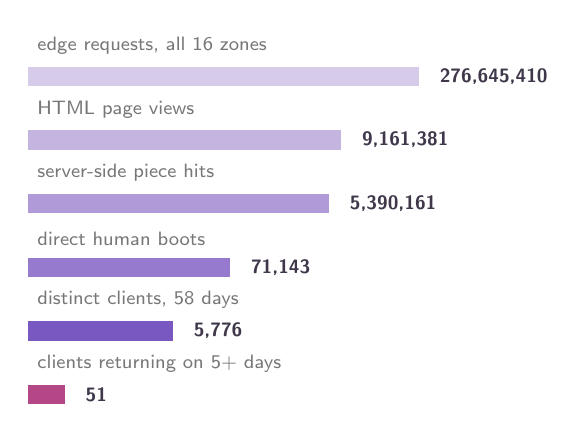
\begin{tikzpicture}[x=1pt,y=1pt]
\definecolor{c1}{RGB}{214,203,232}
\definecolor{c2}{RGB}{196,180,224}
\definecolor{c3}{RGB}{176,155,216}
\definecolor{c4}{RGB}{150,122,206}
\definecolor{c5}{RGB}{122,88,194}
\definecolor{c6}{RGB}{180,72,135}
\foreach \i/\w/\c/\lab/\val in {
  0/141.4/c1/{edge requests, all 16 zones}/{276{,}645{,}410},
  1/113.3/c2/{HTML page views}/{9{,}161{,}381},
  2/108.9/c3/{server-side piece hits}/{5{,}390{,}161},
  3/73.2/c4/{direct human boots}/{71{,}143},
  4/52.5/c5/{distinct clients, 58 days}/{5{,}776},
  5/13.4/c6/{clients returning on 5+ days}/{51}}
{
  \node[anchor=south west, tag] at (0,-\i*23+3.5) {\lab};
  \fill[\c] (0,-\i*23-4.5) rectangle (\w,-\i*23+2.5);
  \node[anchor=west, font=\scriptsize\sffamily\bfseries, text=acdark]
    at (\w+4,-\i*23-1) {\val};
}
\end{tikzpicture}
\caption{The network's year, reduced. Each band is measured by a different instrument (\S\ref{sec:method}). Bar length is $\log_{10}$ of the count, so six orders of magnitude stay visible in one frame. Period is 2026-01-01 to 2026-09-09, except the bottom two bands (2026-07-14 to 2026-09-09). A further 47,839 boots ran inside an iframe and are excluded from the bottom three bands (\S\ref{sec:method-embed}).}
\label{fig:funnel}
\end{figure}

\section{The human layer}
\label{sec:human}

71,143 boots opened the runtime directly --- not inside anybody's
iframe --- between 24~January and 9~September.
Table~\ref{tab:months} breaks them down.

\begin{table}[t]
\centering
\footnotesize
\caption{Direct human boots by month. ``Ran'' is the share whose event trace reached \texttt{running boot}, the point at which the piece is on screen. Clients before July are undercounts (\S\ref{sec:method}) and are omitted. Embedded boots are excluded throughout (\S\ref{sec:method-embed}).}
\label{tab:months}
\vspace{0.35em}
\begin{tabular}{@{}l r r r r@{}}
\toprule
\textbf{Month} & \textbf{Boots} & \textbf{Ran} & \textbf{Mobile} & \textbf{Clients} \\
\midrule
Jan (from 24th) &  2,852 & 64.8\% & --- & --- \\
Feb             & 10,955 & 67.5\% & 26.3\% & --- \\
Mar             &  9,253 & 66.7\% & 41.4\% & --- \\
Apr             & 11,300 & 73.5\% & 38.9\% & --- \\
May             &  8,383 & 72.4\% & 45.8\% & --- \\
Jun             &  8,707 & 74.3\% & 44.8\% & --- \\
Jul             &  6,965 & 85.6\% & 41.1\% & 1,579 \\
Aug             &  9,201 & 81.3\% & 45.9\% & 2,970 \\
Sep (to 9th)    &  3,527 & 72.0\% & 29.5\% & 1,847 \\
\midrule
\textbf{Total}  & \textbf{71,143} & \textbf{73.4\%} & & \\
\bottomrule
\end{tabular}
\end{table}

The striking thing about this table is that nothing happens in it.
Every full month of 2026 sits between 8,383 and 11,300 direct boots.
There is no growth, no decay, and --- once the gallery page of
\S\ref{sec:method-embed} is removed --- no event. The network has run
at roughly 300 human boots a day, every day, for eight months, through
thirteen domain launches, an installation, a native OS release and a
game.

What does move is the client count in the trustworthy window: 1,579 in
July, 2,970 in August, 1,847 in the first nine days of September.
Across the whole 58-day window the runtime was opened directly by
\textbf{5,776 distinct clients in 106 countries}. Flat boots against a
rising client count means the same volume spread across more people:
more strangers, each staying less. That is the shape of a site being
discovered, not of one being used.

The one durable destination is the Danish clock.
\texttt{/laer-klokken} took 22,278 direct boots across the year and
never fell below 2,441 in any full month, peaking at 4,157 in April,
with 998 distinct clients opening it between June and September alone.
It is the only piece in the network with a habit attached to it, and it
is a clock --- an object whose entire proposition is that you look at it
again tomorrow.

The geography follows from that. Table~\ref{tab:geo} ranks by client
rather than by volume, which separates a distributed audience from a
single busy machine: Turkey sits high by boots and nearly nowhere by
clients, because almost all of it is one \ac{} Native OS device polling
from a single address.

\begin{table}[t]
\centering
\footnotesize
\caption{Top countries by distinct client, direct boots, 2026-07-14 to 2026-09-09. 106 countries appear in total.}
\label{tab:geo}
\vspace{0.35em}
\begin{tabularx}{\columnwidth}{@{}Xrr@{\hspace{1.2em}}Xrr@{}}
\toprule
& \textbf{Cl.} & \textbf{Boots} & & \textbf{Cl.} & \textbf{Boots} \\
\midrule
US & 1,220 & 3,296 & NL &  69 & 270 \\
DK &   935 & 7,447 & IN &  66 &  81 \\
NO &   486 &   865 & GB &  59 & 163 \\
CN &   280 &   296 & AR &  52 &  66 \\
SG &   199 &   202 & DE &  51 &  97 \\
FR &   146 &   182 & HK &  51 &  53 \\
BR &   119 &   146 & BD &  49 &  49 \\
\bottomrule
\end{tabularx}
\end{table}

935 Danish clients produced 7,447 boots in 58 days against 3,296 from
1,220 American ones. The clock is the whole of that difference.

Roughly 42\% of direct boots are mobile. The signed-in layer is much
smaller than the identity layer suggests: 2,973 handles are registered,
and 41, 73 and 31 distinct handles appeared in July, August and the
first nine days of September respectively. In its best month the
network was used, while signed in, by 2.5\% of the people who have ever
claimed a name on it.

\section{Arrival}
\label{sec:arrival}

Only about one direct boot in twelve carries an external referrer. What
those referrers are is the most actionable table in the report.

\begin{table}[t]
\centering
\footnotesize
\caption{External referrers by boots, whole year. ``Run'' is the share of arrivals whose trace reached \texttt{running boot}. Rows marked $\ddagger$ deliver every arrival inside an iframe. Sources referring fewer than 30 boots are omitted.}
\label{tab:ref}
\begin{tabularx}{\columnwidth}{@{}X r r r@{}}
\toprule
\textbf{Referrer} & \textbf{Boots} & \textbf{Clients} & \textbf{Run} \\
\midrule
www.google.com          & 926 & 553 & 86\% \\
jas.life                & 886 & 511 & 71\% \\
bing.com                & 504 & 130 & 94\% \\
\textbf{justforfun.io}  & 487 & 437 & \textbf{94\%} \\
mail.google.com         & 454 & 181 & 94\% \\
www.tiktok.com          & 236 & 185 & 78\% \\
google (Android search) & 219 & 139 & 88\% \\
\textbf{cloudhiker.net} & 202 & 179 & 78\% \\
l.instagram.com         & 170 & 105 & 90\% \\
www.facebook.com        & 162 & 119 & \textbf{33\%} \\
www.raster.art$\ddagger$ &  91 &  73 & 45\% \\
opensea.io$\ddagger$    &  87 &  70 & 30\% \\
\textbf{openweird.com}  &  81 &  78 & 86\% \\
github.com              &  76 &  54 & 92\% \\
duckduckgo.com          &  54 &  35 & 96\% \\
tangled.org             &  52 &  39 & 88\% \\
whistlegraph.org        &  46 &  30 & 78\% \\
go.bsky.app             &  33 &  29 & 91\% \\
rhizome.org             &  32 &  26 & 91\% \\
\textbf{pointlesssites.com} & 30 & 24 & 93\% \\
\bottomrule
\end{tabularx}
\end{table}

Read the clients column, not the boots column. \texttt{bing.com} sent
504 boots from 130 clients --- a handful of people reloading, or a
crawler with a browser. \texttt{justforfun.io} sent 487 boots from
\textbf{437 distinct clients}: 437 different people, one visit each,
94\% of whom got a running piece. By that measure it is the single
best-performing external surface the network has, ahead of Google.

\texttt{justforfun.io}, \texttt{cloudhiker.net},
\texttt{openweird.com} and \texttt{pointlesssites.com} are the same
kind of object --- serendipity directories, the ``random interesting
website'' genre that survived the social era by not competing with it.
Alongside them in the referrer tail sit
\texttt{tinytools.directory}, \texttt{dog-house.neocities.org} and
\texttt{sadgrlonline.github.io}: personal link pages and small-web
indexes. Nobody at this project submitted anything to any of them on
purpose.

Where they point is \texttt{nopaint.art}, which is not in
Table~\ref{tab:zones} because its DNS sits outside this Cloudflare
account, and which nonetheless quietly became the network's best
front door. It took 1,238 boots from \textbf{1,069 distinct clients},
essentially all of them landing on \texttt{/}: 431 from
\texttt{justforfun.io}, 76 from \texttt{openweird.com}, 47 from Google,
29 from \texttt{pointlesssites.com}, 14 from a Neocities page, 12 from
Reddit. One piece, one path, no prompt, no login --- and a run rate that
beats the main domain.

Three referrers lose most of what they send.
\texttt{www.facebook.com} arrivals reach graphics initialisation 94\%
of the time and \texttt{running boot} only 33\% of the time: the canvas
appears and they are gone within the second it takes to load the piece.
\texttt{opensea.io} (289 boots, all inside an iframe) and
\texttt{www.raster.art} (140 boots, all embedded) run 57\% and 56\% of
the time, and contribute most of the report's zero-event
records --- boots that registered and then never reported another line.
Embedded playback of a token's artwork is a materially worse experience
than opening the same piece directly, and it is measurable.

\section{Return}
\label{sec:return}

Table~\ref{tab:ret} is the retention picture over the trustworthy
window. It is the least comfortable table here.

\begin{table}[t]
\centering
\footnotesize
\caption{Days active per distinct client, direct boots, 2026-07-14 to 2026-09-09 (58 days).}
\label{tab:ret}
\vspace{0.35em}
\begin{tabularx}{\columnwidth}{@{}X r r r@{}}
\toprule
\textbf{Days active} & \textbf{Clients} & \textbf{Boots} & \textbf{Share of boots} \\
\midrule
1 day       & 5,401 & 10,512 & 63.1\% \\
2--4 days   &   323 &  2,604 & 15.6\% \\
5--9 days   &    33 &  1,035 &  6.2\% \\
10+ days    &    18 &  2,503 & 15.0\% \\
\midrule
\textbf{Total} & \textbf{5,776} & \textbf{16,660} & \\
\bottomrule
\end{tabularx}
\end{table}

93.5\% of the people who opened a piece did so on exactly one day and
never came back. Fifty-one clients --- fifty-one --- returned on five or
more days, and eighteen of those produced 15.0\% of every direct boot
in the window. The network has an audience of nearly six thousand and a
community of about fifty.

The making signals agree. Paintings saved per month ran 46, 47, 67,
39, 38, 23, 78, 142 from January to August --- a real recovery in the
second half, and still under five a day. Chat messages fell from 876 in
March to 38 in August and 5 in the first nine days of September, against
12,449 in the same collection for 2024; mood posts fell from 52 in
March to 13 in August. Hearts, the reaction primitive added in
February, rose steadily to 65 in August. The parts of the network that
ask for a sentence are emptying; the parts that ask for a tap are
holding.

\section{Endpoint health}
\label{sec:health}

\subsection{Boot latency}

Median boot time for direct arrivals held between 3.0 and 4.6 seconds
from March onward, with the 90th percentile between 6.5 and 9.0
seconds. January and February are worse --- p50 10.4~s and 6.6~s ---
because client-side timing then covered module-graph fetches later
moved behind the service worker. For September the figures are
p50~2.98~s and p90~8.32~s. The classical usability threshold
for holding attention is one second for flow and ten seconds for
abandonment~\citep{nielsen1993response}; a tenth of arrivals are at or
past the second of those limits before the instrument makes a sound.

\subsection{Errors and unresolved boots}

Explicit boot errors are rare and concentrated: 1,334 across the year,
of which 520 fell in August. The dominant terminal event is
\texttt{connection error --- retrying}, 514 occurrences since June,
followed by module-load retries. These are network failures on the
module graph, which is the same failure surface addressed by the
service-worker timeout race shipped in September.

A larger category is quieter. In September, 1,213 of 3,601 boots
remain at status \texttt{started}: the document was created and the
completion write never arrived. 299 of them carry zero events at all;
281 stall at \texttt{loading core modules}; 193 recorded
\texttt{running boot} --- meaning the piece did start --- and were never
marked complete. This is a mix of real abandonment and a telemetry
write that does not survive a closing tab, and the two cannot currently
be separated. It is why this report uses ``reached \texttt{running
boot}'' rather than ``status success'' as its completion measure.

On the origin, 1,190 responses in a 3.75-hour sample were 5xx.
They are almost entirely two endpoints: \texttt{/api/macpal-status}
(618) and \texttt{/api/macpal-art} (310) returned 500 continuously,
which extrapolates to roughly six thousand errors a day, with
\texttt{/api/flux} adding 73 503s and \texttt{/api/pruttivox} 15.
Two broken endpoints have been failing on every call, at volume, for
long enough that nobody noticed.

The origin also absorbs a steady scan load --- 488 requests to
\texttt{/wp-admin/index.php} and 261 to \texttt{/wp-login.php} in the
same 3.75 hours --- which is unremarkable in itself and consequential
only because of what it does to the piece ledger.

\subsection{Instrumentation faults}
\label{sec:faults}

Four defects change what can be claimed, and all four are cheap to fix.

\begin{table}[t]
\centering
\footnotesize
\caption{Measurement defects found while assembling this report.}
\label{tab:faults}
\begin{tabularx}{\columnwidth}{@{}>{\raggedright\arraybackslash}p{0.30\columnwidth}>{\raggedright\arraybackslash}X@{}}
\toprule
\textbf{Defect} & \textbf{Consequence} \\
\midrule
Geo headers wrong until 2026-07-14 & No country and no true client IP for the first six months of the year. Fixed in \texttt{9dbe9b83fa}. \\
\addlinespace
\texttt{piece-hits} accepts any slug & The second most-hit ``piece'' of 2026 is \texttt{+CSCOE+/logon.html}, a Cisco VPN exploit probe, at 20,435 hits; \texttt{+webvpn+/index.html} is sixth at 9,802. \\
\addlinespace
KidLisp registry dark & The \texttt{kidlisp} collection last recorded a read on 2026-04-19 and last accepted a new code on 2026-06-17, while \texttt{/api/store-kidlisp} still takes \textasciitilde290 requests every 3.75\,h. Its \texttt{hits} and \texttt{lastAccessed} columns are frozen. \\
\addlinespace
No product analytics & \texttt{shared/posthog-policy.mjs} classifies every endpoint in the system for PostHog, with per-class exclusions. No project token is configured in the repository or the vault. The policy is complete and the instrument was never installed. \\
\bottomrule
\end{tabularx}
\end{table}

The KidLisp gap is the expensive one. KidLisp codes are the artifact
the network was built to pass around~\citep{scudder2026kidlisp}, and
the canonical record of their creation and access has been blind for a
quarter of the year while the codes themselves continue to serve.

\section{Ten openings}
\label{sec:openings}

Ranked by expected effect per hour of work. Each names the measurement
that motivates it.

\textbf{1. Stop polling \texttt{/api/version} at one hertz.}
1,098,386 requests in a day, 57.0\% of the zone, answered 1,159,323
times with an empty 304. A 60-second interval with edge caching, or a
push over the session socket that already exists, removes about
1.08~million requests a day and makes every other number in this report
legible for the first time. Nothing downstream needs second-resolution
build freshness.

\textbf{2. Stop fetching \texttt{handle-colors} over the network.}
315,508 requests a day, 16.4\% of the zone, for a pure function of a
handle called from \texttt{disk.mjs} and \texttt{disk.worker}. Compute
it locally or ship it as an immutable hashed asset. Openings 1 and 2
together are 73.4\% of the top domain's traffic.

\textbf{3. Call \texttt{piece-hit} in process.} lith issues 9,647 HTTP
POSTs to its own public URL in 3.75 hours, out through Cloudflare and
back. It is one function call away. Fix the slug filter in the same
change so the ledger stops recording exploit probes as pieces.

\textbf{4. Fix the two endpoints that fail on every call.}
\texttt{/api/macpal-status} and \texttt{/api/macpal-art} returned 500
to 928 of 928 requests in the sample. Add the alert while you are
there: 5xx rate per endpoint is one Grafana panel, and its absence is
the reason this went unnoticed.

\textbf{5. Restore the KidLisp registry, then read it.} No creation
record since 17~June and no read record since 19~April, for the
language the network is named around. Direct arrivals at a bare \texttt{\$code} fell from 681 in June to 22
in the first nine days of September, and with the registry dark there
is no way to tell whether people stopped making codes or the store
stopped saying so.

\textbf{6. Submit every domain to the serendipity directories.}
\texttt{justforfun.io} delivered 437 distinct clients at a 94\% run
rate without being asked. \texttt{cloudhiker.net},
\texttt{openweird.com}, \texttt{pointlesssites.com} and
\texttt{tinytools.directory} did the same at smaller scale. These are
submission forms, not campaigns; the cost is an afternoon and the
measured conversion beats Google. Submit \texttt{nopaint.art},
\texttt{notepat.com}, \texttt{kidlisp.com}, \texttt{laklok.com} and
\texttt{oskiewar.com} separately, because each is a single-purpose page
of exactly the kind those indexes list.

\textbf{7. Treat \texttt{nopaint.art} as the front door it already
is.} 1,069 distinct clients, one path, no prompt, no login, a better
run rate than the main domain. It is the only surface in the network
that a stranger can succeed at in four seconds. Everything the project
wants a newcomer to find should be reachable from it, and the same
shape --- one piece, one path, no chrome --- should be what every other
piece domain serves at \texttt{/}.

\textbf{8. Give the 5,776 a reason to come back.} 93.5\% of clients
appeared on exactly one day, and the only retention instrument in the
whole record is a push-token collection holding three rows. The
network already knows what works: \texttt{/laer-klokken} held 2,441 to
4,157 boots a month for eight months because a clock is worth opening
again tomorrow. Build the second one, and give people a low-friction
way to be told when it changes.

\textbf{9. Cut p90 boot time below four seconds.} p50 is 2.98~s and
p90 is 8.32~s, and 73.4\% of direct boots reach \texttt{running boot}
against 94\% for the best-converting referrer. Strangers on cold caches
are the gap. The service-worker and immutable-bundle work shipped in
September addresses the module graph; the remaining cost is bios and
its imports, which are still fetched as thirty-two separate files.

\textbf{10. Decide about the empty domains.} \texttt{drvkforlife.com}
served five requests this year and \texttt{oskiewar.com} served one,
for a game with twenty thousand recorded matches. Either point them at
something --- \texttt{oskiewar.com} at the game, per opening 7 --- or let
them lapse. Sixteen zones with two carrying 97.2\% of traffic is not a
network; it is one network and fourteen parked names.

\section{Ethics, privacy, limitations}

No individual is identified in this report. Boot telemetry records a
handle only after authentication resolves, and handles appear here only
as counts. IP addresses were used to count distinct clients and to
separate a single busy machine from a distributed audience; they are
not reproduced, and the shipped data bundle contains no address, no
handle and no user agent string. Geography is reported at country
level, as Cloudflare supplies it. The one client examined
individually --- the Turkish address making 14,366 requests --- is a device
this project operates.

Three limitations bound the conclusions. Distinct-client counts rest on
IP addresses, which conflate households behind a NAT and split mobile
users who roam; they are a floor, not a census. The path-level and
user-agent figures come from a single day, because the free Cloudflare
tier will not answer a wider question, and a single day in early
September may not represent the year. The completion measure (``reached \texttt{running boot}'') cannot
distinguish a boot that failed from a person who left after one second,
which is precisely the ambiguity opening~4 of the telemetry work should
remove. And the direct/embedded split rests on a browser-reported flag
plus a referrer: an always-on display that reports neither would still
be counted as a person, and this report found one such surface only
because its hourly profile was flat at four in the morning.

\section{Conclusion}

The network served 276,645,410 requests and was opened by roughly
5,800 people, fifty-one of whom came back on more than four days. Both
numbers are true, and the distance between them is not a measurement
artifact --- it is a description of the system. Ninety-three percent of
the traffic is the network talking to itself at one hertz, the largest
apparent audience event in the record was a screen in a room, and the
instrument that could have told us either of those things was never
installed.

What the data does not show is a demand problem. About a hundred new machines a day, three hundred boots, have arrived
every day for eight months --- from search, from a Danish clock, and most
efficiently from a handful of volunteer indexes of interesting websites
that nobody here has ever contacted.
When they arrive at a single-purpose page they succeed nine times in
ten; when they arrive at a prompt, seven times in ten; when they arrive
inside a marketplace iframe, one time in three. What the data does show
is a returning problem, and a clock in Denmark is the only thing in
eight months that has solved it. The openings above are ordered by that
difference. Nine of the ten cost less than a day.

\section{Appendix: the router's year}
\label{sec:appendix}

Table~\ref{tab:pieces} sets the two ledgers side by side. The left panel
is every request the HTML router answered for a slug, crawlers included;
the right panel is the same period counted in humans who actually ran
the piece. They disagree about almost everything, and the disagreement
is the report in miniature.

\begin{table}[h]
\centering
\footnotesize
\caption{Left: top slugs by server-side hit, 2025-12-31 to 2026-09-09, from the \texttt{piece-hits} ledger. Right: top named destinations by distinct human client, 2026-06-01 to 2026-09-09, from boot telemetry. Rows marked $\dagger$ are exploit probes the ledger records as pieces (\S\ref{sec:faults}).}
\label{tab:pieces}
\vspace{0.35em}
\begin{tabular}{@{}l r@{\hspace{1.1em}}l r r@{}}
\toprule
\textbf{Slug} & \textbf{Hits} & \textbf{Piece} & \textbf{Cl.} & \textbf{Boots} \\
\midrule
\texttt{prompt}            & 4,994,635 & \texttt{laer-klokken} & 998 & 8,654 \\
\texttt{+CSCOE+/}$\dagger$ &    20,435 & \texttt{starfield}    & 290 &   431 \\
\texttt{laer-klokken}      &    19,800 & \texttt{notepat}      & 182 &   231 \\
\texttt{nopaint}           &    11,093 & \texttt{nopaint}      & 126 &   177 \\
\texttt{notepat}           &    10,981 & \texttt{laklok}       & 112 &   499 \\
\texttt{+webvpn+/}$\dagger$&     9,802 & \texttt{chat}         &  86 &   115 \\
\texttt{\$bop}             &     3,775 & \texttt{kidlisp}      &  55 &    88 \\
\texttt{\$4xa}             &     3,172 & \texttt{r8dio}        &  52 &   102 \\
\texttt{\$ceo}             &     2,927 & \texttt{baktok}       &  49 &    78 \\
\texttt{\$roz}             &     2,858 & \texttt{prutti}       &  42 &    56 \\
\texttt{\$pie}             &     2,798 & \texttt{processing}   &  41 &    44 \\
\texttt{\$cow}             &     2,517 & \texttt{list}         &  35 &    51 \\
\texttt{starfield}         &     2,094 & \texttt{@jeffrey}     &  30 &    40 \\
\texttt{\$nsh}             &     1,940 & \texttt{girlfriend}   &  26 &    43 \\
\texttt{api/.env}$\dagger$ &     1,817 & \texttt{dannom}       &  16 &    36 \\
\bottomrule
\end{tabular}
\end{table}

Three readings. First, \texttt{prompt} --- the default piece, served for
every bare load of the domain --- is 92.7\% of the ledger's 5,390,161
recorded hits, which makes the ledger a measure of the front page and
not of the catalogue. Second, three of the fifteen most-hit slugs of
2026 are exploit probes: \texttt{+CSCOE+/logon.html} and
\texttt{+webvpn+/index.html} are Cisco VPN reconnaissance, and
\texttt{api/.env} is a credentials sweep that has run every day since
1~January. Each of them out-ranks every KidLisp code in the system.
Third, the human panel is two orders of magnitude smaller and ranks
differently: \texttt{starfield}, which does not appear in the ledger's
top twelve, is the second most-visited named piece by real people, and
\texttt{laklok} draws 4.5 boots per client --- the highest repeat rate of
any destination outside the clock itself.

One more distribution belongs here, because it is the clearest picture
of how the network is actually addressed. Sorting all
71,143 direct boots by the shape of the entry URL gives 38,154
arrivals at the root or \texttt{/prompt} (53.6\%), 30,439 at a named
piece (42.8\%), 1,620 at a bare KidLisp \texttt{\$code} (2.3\%), and
930 at a \texttt{@handle} page (1.3\%). Two of those numbers are
uncomfortable. A person opens somebody else's KidLisp code by its
three-letter name about six times a day across the entire network:
outside the gallery iframe, the sharing gesture the language was
designed around is almost unused. And the \texttt{@handle} page, the
one surface that would make a person findable, is 1.3\% of arrivals in
a system holding 2,973 registered names. The named-piece share does
grow --- 32\% of February's direct boots, 58\% of September's --- which
is the report's one unambiguous trend: people increasingly arrive at a
thing rather than at a prompt.

The practical consequence is opening~3. A ledger that cannot tell a
piece from a probe cannot be used to decide what to build next, which
is the only reason to keep it.

\bibliographystyle{plainnat}
\setlength{\bibsep}{1.2pt plus 0.2ex}
{\footnotesize
\bibliography{references}
}

\end{document}
